% Unofficial University of Cambridge Poster Template
% https://github.com/andiac/gemini-cam
% a fork of https://github.com/anishathalye/gemini
% also refer to https://github.com/k4rtik/uchicago-poster

\documentclass[final]{beamer}

% ====================
% Packages
% ====================

\usepackage[T1]{fontenc}
\usepackage{lmodern}
\usepackage[size=custom,width=120,height=72,scale=1.0]{beamerposter}
\usetheme{gemini}
\usecolortheme{cam}
\usepackage{graphicx}
\usepackage{booktabs}
\usepackage[numbers]{natbib}
\usepackage{tikz}
\usepackage{pgfplots}
\pgfplotsset{compat=1.14}
\usepackage{anyfontsize}

% ====================
% Lengths
% ====================

% If you have N columns, choose \sepwidth and \colwidth such that
% (N+1)*\sepwidth + N*\colwidth = \paperwidth
\newlength{\sepwidth}
\newlength{\colwidth}
\setlength{\sepwidth}{0.025\paperwidth}
\setlength{\colwidth}{0.3\paperwidth}

\newcommand{\separatorcolumn}{\begin{column}{\sepwidth}\end{column}}

% ====================
% Title
% ====================

\title{Dinkelbach Algorithm for SBPO Challenge 2025}

\author{Santiago Cifuentes \inst{1} \and Ignacio Oromendia \inst{1} \and Luciana Skakovsky \inst{1}}

\institute[shortinst]{\inst{1} FCEN - Universidad de Buenos Aires }

% ====================
% Footer (optional)
% ====================

\footercontent{
  \href{https://www.example.com}{https://www.example.com} \hfill
  SBPO 2025 \hfill
  \href{mailto:alyssa.p.hacker@example.com}{alyssa.p.hacker@example.com}}
% (can be left out to remove footer)

% ====================
% Logo (optional)
% ====================

% use this to include logos on the left and/or right side of the header:
% \logoright{\includegraphics[height=7cm]{logo1.pdf}}
% \logoleft{\includegraphics[height=7cm]{logo1.pdf}}

% ====================
% Body
% ====================

\begin{document}

% Refer to https://github.com/k4rtik/uchicago-poster
% logo: https://www.cam.ac.uk/brand-resources/about-the-logo/logo-downloads
\addtobeamertemplate{headline}{}
{
    \begin{tikzpicture}[remember picture,overlay]
      \node [anchor=north west, inner sep=3cm] at ([xshift=0.0cm,yshift=1.0cm]current page.north west)
      {
\includegraphics[height=4.5cm]{logos/cambridge-reversed-color-logo.eps}}; 
    \end{tikzpicture}
}

\begin{frame}[t]
\begin{columns}[t]
\separatorcolumn

\begin{column}{\colwidth}

  \begin{block}{The Problem}

    In warehouse operations, picking each order individually is inefficient. Instead, we group compatible orders into \textbf{waves} so that their items can be collected together through shorter and more efficient routes. The goal is to decide which orders should form the next wave to maximize \textbf{picking productivity} — that is, to collect as many products as possible while visiting as few aisles as needed.

    Let:
\begin{itemize}
    \item $O$ = set of all pending orders.
    \item $I_o$ = set of items requested in order $o \in O$.
    \item $A$ = set of aisles in the warehouse.
    \item $A_i \subseteq A$ = aisles containing item $i$.
    \item $u_{oi}$ = units of item $i$ requested by order $o$.
    \item $u_{ai}$ = units of item $i$ available in aisle $a$.
    \item $LB, UB$ = lower and upper bounds on the total number of items in the wave.
\end{itemize}

We want to select:
\[
O' \subseteq O \quad \text{(orders in the wave)}, \qquad
A' \subseteq A \quad \text{(aisles to visit)}
\]
so as to maximize the ratio between collected units and visited aisles:

\[
\max_{O',A'} \; \frac{\displaystyle\sum_{o \in O'} \sum_{i \in I_o} u_{oi}}{|A'|}
\]

subject to:
\begin{align}
    &\sum_{o \in O'} \sum_{i \in I_o} u_{oi} \ge LB \tag{1}\\[3pt]
    &\sum_{o \in O'} \sum_{i \in I_o} u_{oi} \le UB \tag{2}\\[3pt]
    &\sum_{o \in O'} u_{oi} \le \sum_{a \in A'} u_{ai}, \quad \forall i \in I_o, \; o \in O' \tag{3}
\end{align}

A pair $(O',A')$ satisfying (1)--(3) defines a feasible wave, and the optimal wave maximizes the productivity ratio above.
  \end{block}

  \begin{block}{An Exact Parametric Approach}

    Nam vulputate nunc felis, non condimentum lacus porta ultrices. Nullam sed
    sagittis metus. Etiam consectetur gravida urna quis suscipit.

    \begin{itemize}
      \item \textbf{Mauris tempor} risus nulla, sed ornare
      \item \textbf{Libero tincidunt} a duis congue vitae
      \item \textbf{Dui ac pretium} morbi justo neque, ullamcorper
    \end{itemize}

    Eget augue porta, bibendum venenatis tortor.

  \end{block}

  

\end{column}

\separatorcolumn

\begin{column}{\colwidth}

  \begin{block}{Warm start}

    The Dinkelbach algorithm can benefit from a high quality initial solution, and thus we consider two simple greedy strategies to obtain them.
    The first one prioritizes picking aisles of a big \textit{size} (i.e. those $a \in A$ that maximize $\sum_{i \in I_o} u_{ai}$) while the second one prioritizes aisles
    with high \textit{diversity} (i.e. those $a \in A$ that maximize $|\{i \in I_o : u_{ai} > 0\}|$). As seen in Figure~\ref{fig:aisles_greedy} optimal solutions have these type of aisles.
    
    \begin{figure}
      \centering
      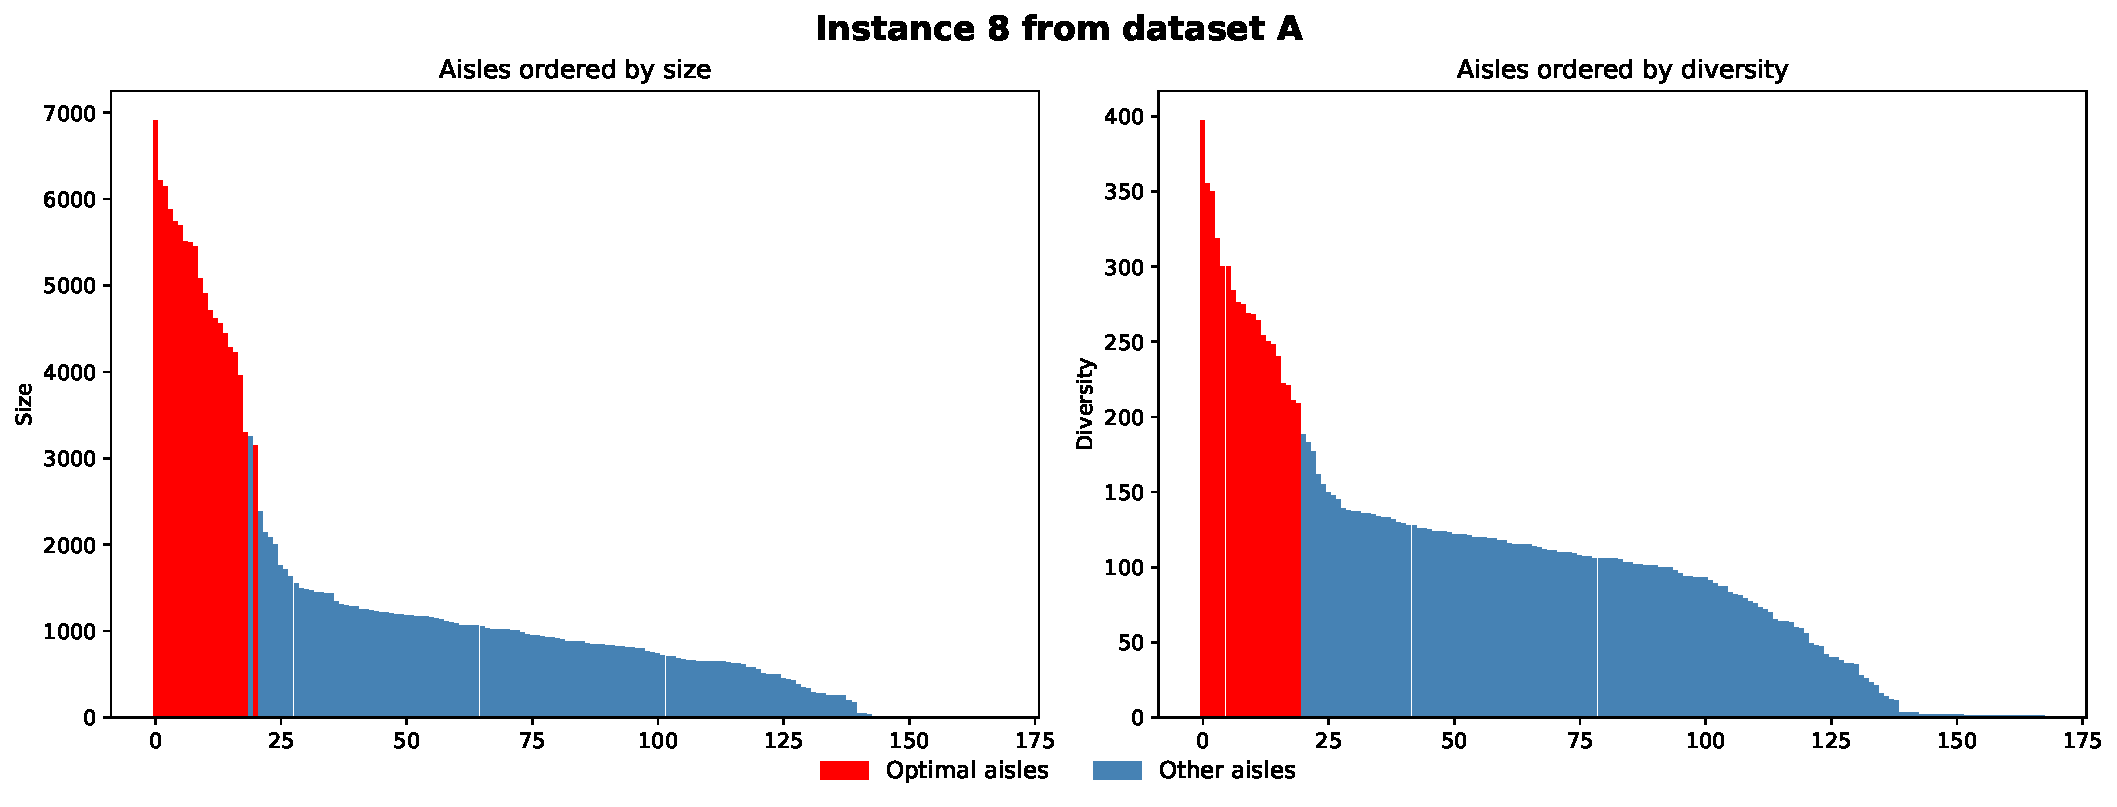
\includegraphics[width=0.8\textwidth]{greedy_instance_a.pdf}
      \caption{Aisles sorted by size and diversity and optimal aisles for instance 8 from dataset A.}
      \label{fig:aisles_greedy}
    \end{figure}

    \begin{columns}
  \begin{column}{0.45\textwidth}
  \justify
  Our algorithm fixes, for each possible $k$, the first $k$ aisles sorted based on each of these two criteria, and then picks orders greedily sorting them by size. Our implementation is efficient with complexity almost linear in the input size,
    and usually finds solutions 10\%-close to the optimal one in the order of seconds, as can be seen in Figure~\ref{fig:greedy_vs_optimal}. In most cases the greedy approach based on diversity beats the one based on size.
  \end{column}
  \begin{column}{0.55\textwidth}  %%<--- here
  \begin{center}
        \begin{figure}
        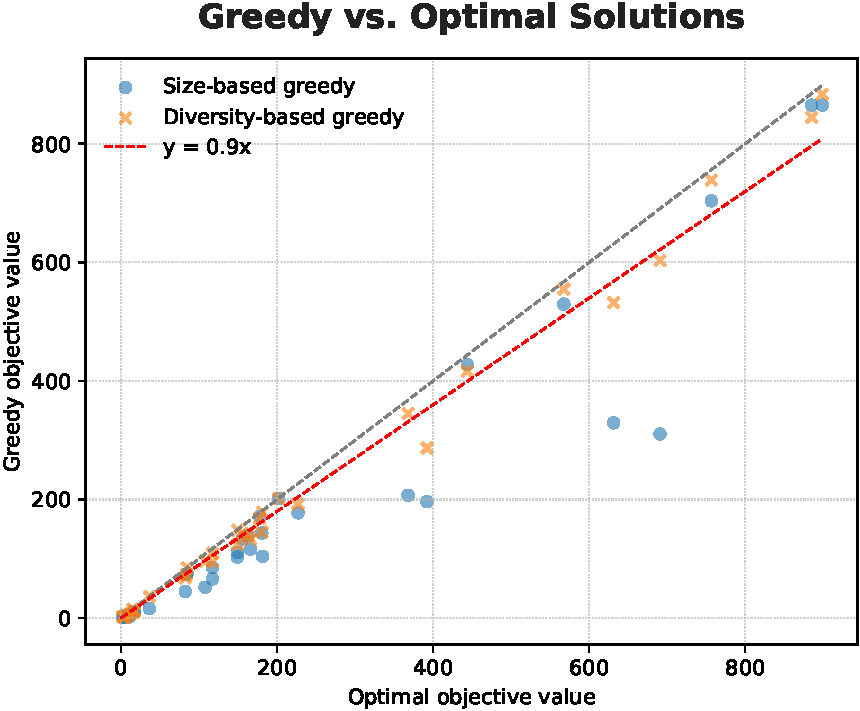
\includegraphics{greedy_vs_optimal.pdf}
        \caption{Comparison between the optimal values and the results given by the greedy algorithms.}
        \label{fig:greedy_vs_optimal}
      \end{figure}
    \end{center}
     \end{column}
  \end{columns}


    
  \end{block}

  \begin{block}{Fusce aliquam magna velit}

    Et rutrum ex euismod vel. Pellentesque ultricies, velit in fermentum
    vestibulum, lectus nisi pretium nibh, sit amet aliquam lectus augue vel
    velit. Suspendisse rhoncus massa porttitor augue feugiat molestie. Sed
    molestie ut orci nec malesuada. Sed ultricies feugiat est fringilla
    posuere.

\vspace{1em}

  \end{block}

  \begin{block}{Nam cursus consequat egestas}

    Nulla eget sem quam. Ut aliquam volutpat nisi vestibulum convallis. Nunc a
    lectus et eros facilisis hendrerit eu non urna. Interdum et malesuada fames
    ac ante \textit{ipsum primis} in faucibus. Etiam sit amet velit eget sem
    euismod tristique. Praesent enim erat, porta vel mattis sed, pharetra sed
    ipsum. Morbi commodo condimentum massa, \textit{tempus venenatis} massa
    hendrerit quis. Maecenas sed porta est. Praesent mollis interdum lectus,
    sit amet sollicitudin risus tincidunt non.

    Etiam sit amet tempus lorem, aliquet condimentum velit. Donec et nibh
    consequat, sagittis ex eget, dictum orci. Etiam quis semper ante. Ut eu
    mauris purus. Proin nec consectetur ligula. Mauris pretium molestie
    ullamcorper. Integer nisi neque, aliquet et odio non, sagittis porta justo.

    \begin{itemize}
      \item \textbf{Sed consequat} id ante vel efficitur. Praesent congue massa
        sed est scelerisque, elementum mollis augue iaculis.
        \begin{itemize}
          \item In sed est finibus, vulputate
            nunc gravida, pulvinar lorem. In maximus nunc dolor, sed auctor eros
            porttitor quis.
          \item Fusce ornare dignissim nisi. Nam sit amet risus vel lacus
            tempor tincidunt eu a arcu.
          \item Donec rhoncus vestibulum erat, quis aliquam leo
            gravida egestas.
        \end{itemize}
      \item \textbf{Sed luctus, elit sit amet} dictum maximus, diam dolor
        faucibus purus, sed lobortis justo erat id turpis.
      \item \textbf{Pellentesque facilisis dolor in leo} bibendum congue.
        Maecenas congue finibus justo, vitae eleifend urna facilisis at.
    \end{itemize}

  \end{block}

\end{column}

\separatorcolumn

\begin{column}{\colwidth}

  \begin{exampleblock}{A highlighted block containing some math}

    A different kind of highlighted block.

    $$
    \int_{-\infty}^{\infty} e^{-x^2}\,dx = \sqrt{\pi}
    $$

    Interdum et malesuada fames $\{1, 4, 9, \ldots\}$ ac ante ipsum primis in
    faucibus. Cras eleifend dolor eu nulla suscipit suscipit. Sed lobortis non
    felis id vulputate.

    \heading{A heading inside a block}

    Praesent consectetur mi $x^2 + y^2$ metus, nec vestibulum justo viverra
    nec. Proin eget nulla pretium, egestas magna aliquam, mollis neque. Vivamus
    dictum $\mathbf{u}^\intercal\mathbf{v}$ sagittis odio, vel porta erat
    congue sed. Maecenas ut dolor quis arcu auctor porttitor.

    \heading{Another heading inside a block}

    Sed augue erat, scelerisque a purus ultricies, placerat porttitor neque.
    Donec $P(y \mid x)$ fermentum consectetur $\nabla_x P(y \mid x)$ sapien
    sagittis egestas. Duis eget leo euismod nunc viverra imperdiet nec id
    justo.

  \end{exampleblock}

  \begin{block}{Nullam vel erat at velit convallis laoreet}

    Class aptent taciti sociosqu ad litora torquent per conubia nostra, per
    inceptos himenaeos. Phasellus libero enim, gravida sed erat sit amet,
    scelerisque congue diam. Fusce dapibus dui ut augue pulvinar iaculis.

    \begin{table}
      \centering
      \begin{tabular}{l r r c}
        \toprule
        \textbf{First column} & \textbf{Second column} & \textbf{Third column} & \textbf{Fourth} \\
        \midrule
        Foo & 13.37 & 384,394 & $\alpha$ \\
        Bar & 2.17 & 1,392 & $\beta$ \\
        Baz & 3.14 & 83,742 & $\delta$ \\
        Qux & 7.59 & 974 & $\gamma$ \\
        \bottomrule
      \end{tabular}
      \caption{A table caption.}
    \end{table}

    Donec quis posuere ligula. Nunc feugiat elit a mi malesuada consequat. Sed
    imperdiet augue ac nibh aliquet tristique. Aenean eu tortor vulputate,
    eleifend lorem in, dictum urna. Proin auctor ante in augue tincidunt
    tempor. Proin pellentesque vulputate odio, ac gravida nulla posuere
    efficitur. Aenean at velit vel dolor blandit molestie. Mauris laoreet
    commodo quam, non luctus nibh ullamcorper in. Class aptent taciti sociosqu
    ad litora torquent per conubia nostra, per inceptos himenaeos.

    Nulla varius finibus volutpat. Mauris molestie lorem tincidunt, iaculis
    libero at, gravida ante. Phasellus at felis eu neque suscipit suscipit.
    Integer ullamcorper, dui nec pretium ornare, urna dolor consequat libero,
    in feugiat elit lorem euismod lacus. Pellentesque sit amet dolor mollis,
    auctor urna non, tempus sem.

  \end{block}

  \begin{block}{References}

    \nocite{*}
    \footnotesize{\bibliographystyle{plainnat}\bibliography{poster}}

  \end{block}

\end{column}

\separatorcolumn
\end{columns}
\end{frame}

\end{document}
